\documentclass[3p, authoryear]{elsarticle} %review=doublespace preprint=single 5p=2 column
%%% Begin My package additions %%%%%%%%%%%%%%%%%%%
\usepackage[hyphens]{url}

  \journal{Submitted to Journal} % Sets Journal name


\usepackage{lineno} % add
\providecommand{\tightlist}{%
  \setlength{\itemsep}{0pt}\setlength{\parskip}{0pt}}

\usepackage{graphicx}
%%%%%%%%%%%%%%%% end my additions to header

\usepackage[T1]{fontenc}
\usepackage{lmodern}
\usepackage{amssymb,amsmath}
\usepackage{ifxetex,ifluatex}
\usepackage{fixltx2e} % provides \textsubscript
% use upquote if available, for straight quotes in verbatim environments
\IfFileExists{upquote.sty}{\usepackage{upquote}}{}
\ifnum 0\ifxetex 1\fi\ifluatex 1\fi=0 % if pdftex
  \usepackage[utf8]{inputenc}
\else % if luatex or xelatex
  \usepackage{fontspec}
  \ifxetex
    \usepackage{xltxtra,xunicode}
  \fi
  \defaultfontfeatures{Mapping=tex-text,Scale=MatchLowercase}
  \newcommand{\euro}{€}
\fi
% use microtype if available
\IfFileExists{microtype.sty}{\usepackage{microtype}}{}
\usepackage{natbib}
\bibliographystyle{apalike}
\usepackage{longtable,booktabs,array}
\usepackage{calc} % for calculating minipage widths
% Correct order of tables after \paragraph or \subparagraph
\usepackage{etoolbox}
\makeatletter
\patchcmd\longtable{\par}{\if@noskipsec\mbox{}\fi\par}{}{}
\makeatother
% Allow footnotes in longtable head/foot
\IfFileExists{footnotehyper.sty}{\usepackage{footnotehyper}}{\usepackage{footnote}}
\makesavenoteenv{longtable}
\usepackage{graphicx}
\ifxetex
  \usepackage[setpagesize=false, % page size defined by xetex
              unicode=false, % unicode breaks when used with xetex
              xetex]{hyperref}
\else
  \usepackage[unicode=true]{hyperref}
\fi
\hypersetup{breaklinks=true,
            bookmarks=true,
            pdfauthor={},
            pdftitle={The Effects of Mode Choice Model Consistency between Activity-based Models and Microsimulation Tools},
            colorlinks=false,
            urlcolor=blue,
            linkcolor=magenta,
            pdfborder={0 0 0}}
\urlstyle{same}  % don't use monospace font for urls

\setcounter{secnumdepth}{5}
% Pandoc toggle for numbering sections (defaults to be off)

% Pandoc citation processing

% Pandoc header
\usepackage{booktabs}
\usepackage{booktabs}
\usepackage{longtable}
\usepackage{array}
\usepackage{multirow}
\usepackage{wrapfig}
\usepackage{float}
\usepackage{colortbl}
\usepackage{pdflscape}
\usepackage{tabu}
\usepackage{threeparttable}
\usepackage{threeparttablex}
\usepackage[normalem]{ulem}
\usepackage{makecell}
\usepackage{xcolor}



\begin{document}
\begin{frontmatter}

  \title{The Effects of Mode Choice Model Consistency between Activity-based Models and Microsimulation Tools}
    \author[Brigham Young University]{Christopher Day\corref{1}}
   \ead{christophersday@gmail.com} 
    \author[Brigham Young University]{Gregory Macfarlane}
   \ead{christophersday@gmail.com} 
      \address[Brigham Young University]{Civil and Environmental Engineering Department, 430 Engineering Building, Provo, Utah 84602}
      \cortext[1]{Corresponding Author}
    \cortext[2]{Present affiliation: some nice job}
  
  \begin{abstract}
  This is where the abstract should go.
  \end{abstract}
   \begin{keyword} Accessibility Passive Data Location Choice\end{keyword}
 \end{frontmatter}

\hypertarget{intro}{%
\section{Question}\label{intro}}

In recent years, there has been variation in how the mode choice is estimated within activity-based travel demand modeling. Originally, \citet{bhat1999activity} stated that travel demand models should use individual trips as the primary unit of analysis, and to calculate mode at a trip level. More recently, \citet{eluru2010econometric} developed a joint multiple discrete continuous extreme value (MDCEV) framework to model the individual's mode choice (among other decisions). \citet{hasnine2021tour} listed differing estimation techniques found in activity-based models, some of which include tour-based modeling, nested model structures, iterative and dynamic processes, and simply calculating the mode choice elsewhere and feeding it in as an input. Variation amoung activity-based models has always existed.

Like with activity-based models, mode choice estimation in microsimulation tools is not universal. \citet{w2016multi} explain that mode choice in MATSim is chosen using the Charypar-Nagel Utility Function, where agents pick the best alternative based on their uniquely calculated utility score. Alternatively, \citet{ciari2008new} proposed introducing multinomial logit models on the subtour level to increase mode choice estimation accuracy in MATSim. In addition, BEAM originally used a Latent Class Choice Model as its mode choice structure, but then switched to a simple multinomial logit model. Alternatively, \citet{barth2020evaluating} proposed that BEAM implements a fundamental influencing factor (FIF) mode choice model instead. As can be seen with MATSim and BEAM, no current common ground has been established in mode choice model structure among microsimulation tools.

Since there is no way to model human behavior perfectly, it does not seem ideal to develop one universal technique to estimating mode choice. However, a useful advancement in travel demand modeling could be to align the internal structure of mode choice in microsimulation with mode choice in activity-based models. Oftentimes, the outputs of activity-based models are used as the inputs to microsimulation tools. Yet, the way mode choice is estimated in a microsimulation tool rarely matches that of its parent activity-based model. This heterogeneity of estimation between models may lead to increased variability in the final microsimulation results.

We hypothesize that a microsimulation tool with a mode choice structure that mimics that of its parenting activity-based model more accurately simulates the distribution of mode choice across a population. In addition, we explore which population characteristics within the mode choice model has the most significant effect in estimating realistic results.

\hypertarget{methods}{%
\section{Methods}\label{methods}}

In our research, the input population used to model behavior corresponds to individuals in the Salt Lake City, Utah, US Region. The activity-based model used to generate the microsimulation input data is ActivitySim \citep{activitysim}. The microsimulation tool used to generate travel behavior data is BEAM \citep{beam}.

ActivitySim implements a multifaceted mode choice model that is dependent on trip, tour, and purpose. One model determines the primary mode for each tour and a separate model determines the mode for each trip. In addition, each modal decision is dependent on the current tour purpose value. Contrastingly, BEAM's default mode choice structure uses a simple multinomial logit model, independent of tour purpose value. Therefore, in order to test our hypothesis, we aligned the mode choice structure of BEAM (a microsimulation tool) with that of ActivitySim (an activity-based model).

To closely align the mode choice structure of BEAM with ActivitySim, we changed much about the code structure inside of BEAM. More specifically, we wrote code that forced modal decisions to be based on tour purpose values. We also implemented the use of ActivitySim's path, person, and location utility parameter values to calculate modal alternative probabilities. These simple steps allowed us to create consistency between an activity-based model and a microsimulation tool.

To test the effectiveness of our calibrated mode choice model, we conducted five different test scenarios within BEAM and compared their outputs with eachout. Each test scenario that we simulated used a multinomial logit function to determine modal probabilities. Although all used a multinomial logit function, each scenario used a different utility function to predict behavior.

The first sceneario we ran used the default BEAM structure. This represented a model with an inconsistent mode choice structure \eqref{eq:label1}. The next three scenarios we ran used a purpose based model with part of ActivitySim's utility function (either using the path \eqref{eq:label2}, person \eqref{eq:label3}, or location type \eqref{eq:label4} variables). These represented models with semi-consistent mode choice structures. The last scenario we ran used a pupose based model with ActivitySim's complete utility function. This represented a model with a consistent mode choice structure \eqref{eq:label5}. Simplified versions of the utility function used in each of the scenarios can be seen in the following equations.\\

\emph{Eq 1: BEAM's Default Utility Equation}

\begin{equation}
  V_j = ASC_j + \beta_{c}(c) + \beta_{t}(t) + \beta_{xfer}(xfer) \label{eq:label1}
\end{equation}

where

\begin{itemize}
\tightlist
\item
  \(j\) is the modal alternative,
\item
  \(c\) is the cost,
\item
  \(t\) is the travel time, and
\item
  \(xfer\) is the number of transfers.
\end{itemize}

\emph{Eq 2: Utility Equation using ActivitySim's Path Variables}

\begin{equation}
  V_j = \beta_{t_v}(t_v) + \beta_{t_w}(t_w) + \beta_{t_e}(t_e) + \beta_{tr_p}(tr_p) + \beta_{xfer}(xfer) + \beta_{w_{dis}}(w_{dis}) + \\ \beta_{b_{dis}}(b_{dis}) + \beta_{d_{dis}}(d_{dis}) \label{eq:label2}
\end{equation}

where

\begin{itemize}
\tightlist
\item
  \(j\) is the modal alternative,
\item
  \(t_v\) is the in vehicle travel time (mins),
\item
  \(t_w\) is the wait time (mins),
\item
  \(t_e\) is the egress time (mins),
\item
  \(tr_p\) is the proximity to transit (miles),
\item
  \(xfer\) is the number of transfers,
\item
  \(w_{dis}\) is the walk distance (miles),
\item
  \(b_{dis}\) is the bike distance (miles),
\item
  \(d_{dis}\) is the drive distance (miles),
\item
  \(\beta_{tr_p}\) differs between origin/destination and length, and
\item
  \(\beta_{w_{dis}}\), \(\beta_{b_{dis}}\), and \(\beta_{d_{dis}}\) differ between lengths.
\item
  \emph{Note:} All \(\beta\) values differ between mode and tour purpose.
\end{itemize}

\emph{Eq 3: Utility Equation using ActivitySim's Person Variables}

\begin{equation}
  V_j = ASC_{auto} +  \beta_{c}(c) + \beta_{ag}(ag) \label{eq:label3}
\end{equation}

where

\begin{itemize}
\tightlist
\item
  \(j\) is the modal alternative,
\item
  \(ASC_{auto}\) is the alternative specific constant that differs between modal alternative and auto ownership dependency,
\item
  \(c\) is the cost, and
\item
  \(ag\) is the age grouping (if the person is between 0-10 or 16-19 years old).
\item
  \emph{Note:} All \(\beta\) values differ between mode and tour purpose.
\end{itemize}

\emph{Eq 4: Utility Equation using ActivitySim's Location Variables}

\begin{equation}
  V_j = \beta_{zdi}(zdi) + \beta_{cbd}(cbd) \label{eq:label4}
\end{equation}

where

\begin{itemize}
\tightlist
\item
  \(j\) is the modal alternative
\item
  \(zdi\) is the zonal density index,
\item
  \(cbd\) is a classifier for zones labeled as central business district, and
\item
  \(\beta_{zdi}\) differs between origin/destination.
\item
  \emph{Note:} All \(\beta\) values differ between mode and tour purpose.
\end{itemize}

\emph{Eq 5: Utility Equation using All of ActivitySim's Variables}

\begin{equation}  
  V_j = Eq:2 + Eq:3 + Eq:4 \label{eq:label5}
\end{equation}

where

\begin{itemize}
\tightlist
\item
  \(j\) is the modal alternative.
\end{itemize}

\hypertarget{findings}{%
\section{Findings}\label{findings}}

The findings of our study are gathered from the events files generated by BEAM foreach scenario run. The events file stores all the decisions made by all individuals during the simulation, including their mode choice decisions. Using the events files, each model's modal shares were thus calculated. To thouroughly understand the affect that each model had on modal shares, modal shares dependent on different variables were calculated. Specifically, the following three modal share outputs were created:

\begin{enumerate}
\def\labelenumi{\arabic{enumi}.}
\tightlist
\item
  Total Modal Share
\item
  Modal Share based on Vehicle Ownership
\item
  Modal Share based on Tour Purpose
\end{enumerate}

The modal share in general describes the percentage of individuals in the simulattion that chose each modal alternatives. A total of 9 modal alternatives were given to the agents:

\begin{enumerate}
\def\labelenumi{\arabic{enumi}.}
\tightlist
\item
  Car
\item
  Drive Transit
\item
  Ride Hail
\item
  Ride Hail Pooled
\item
  Ride Hail Tranist
\item
  Shared 2 Ride
\item
  Shared 3+ Ride
\item
  Walk
\item
  Walk Transit
\end{enumerate}

Comparing the modal share of each of the models with the actual modal share of the region allows one to determine the optimal mode choice structure. In the following comparison, the variable \emph{WFRC} represents the actual modal share of the region.

\hypertarget{total-modal-share}{%
\subsection{Total Modal Share}\label{total-modal-share}}

The total modal share simply describes the total division of mode choice alternatives for the entire population. The following figure shows the total modal share.

\begin{figure}
\centering
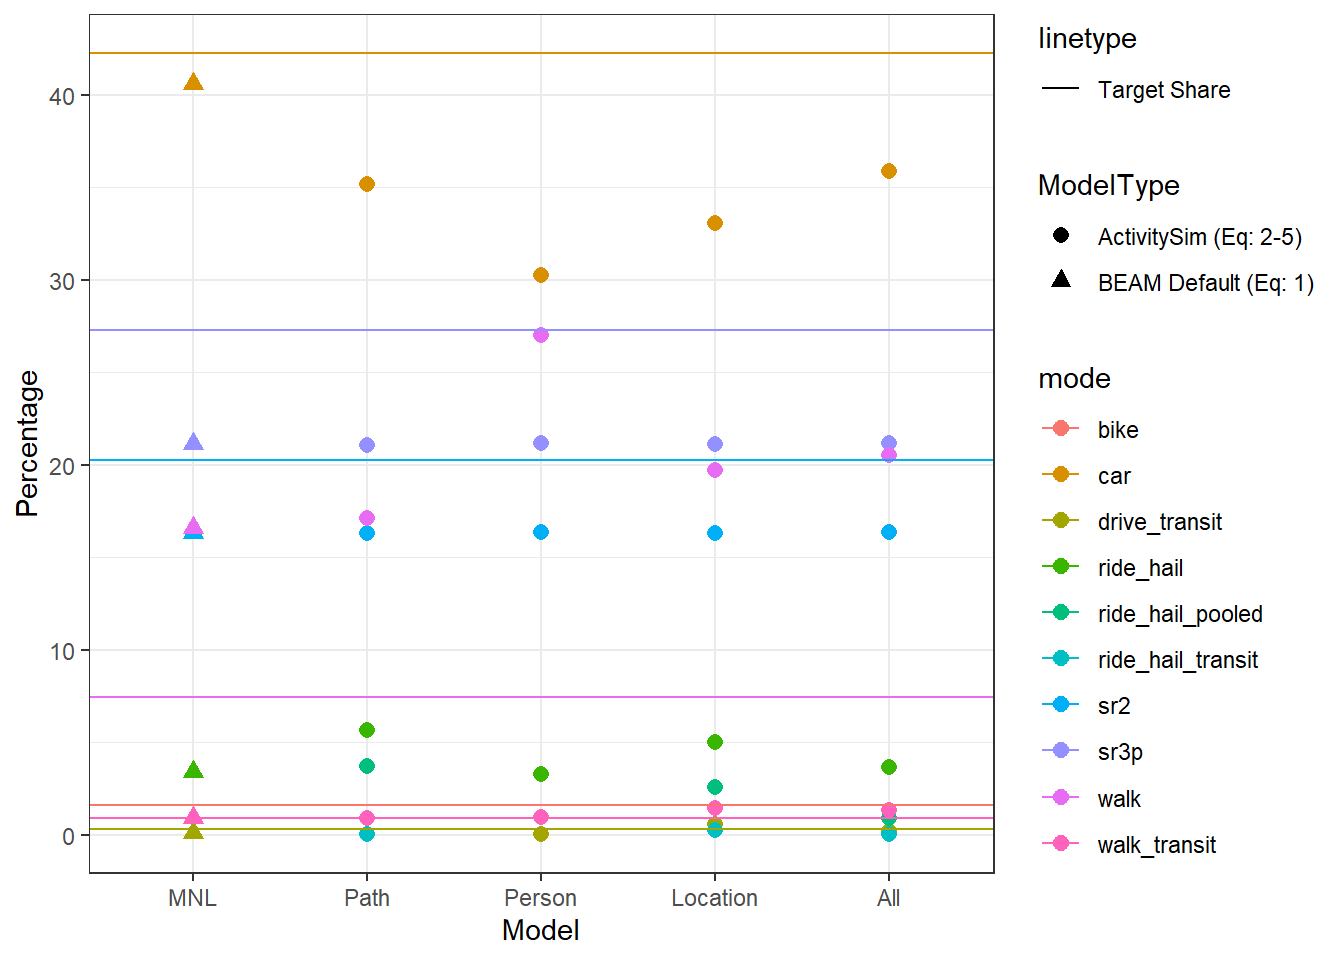
\includegraphics{mode_choice_calibration_files/figure-latex/unnamed-chunk-1-1.pdf}
\caption{\label{fig:unnamed-chunk-1}The Total Modal Split of each Scenario compared with Real World Data.}
\end{figure}

By examining the graph above, it can clearly be seen that the MNL model provides the car modal share closest to that of the actual region . Although this is true, the ALL model provides a closer walk modal share than the rest. The other modal alternatives all seem relatively similar.

\hypertarget{modal-share-by-vehicle-ownership}{%
\subsection{Modal Share by Vehicle Ownership}\label{modal-share-by-vehicle-ownership}}

The modal share by vehicle ownership provides a more detailed view of how the modes are distributed across the population based on their vehicle ownership status. The following figure shows the modal share by vehicle ownership.

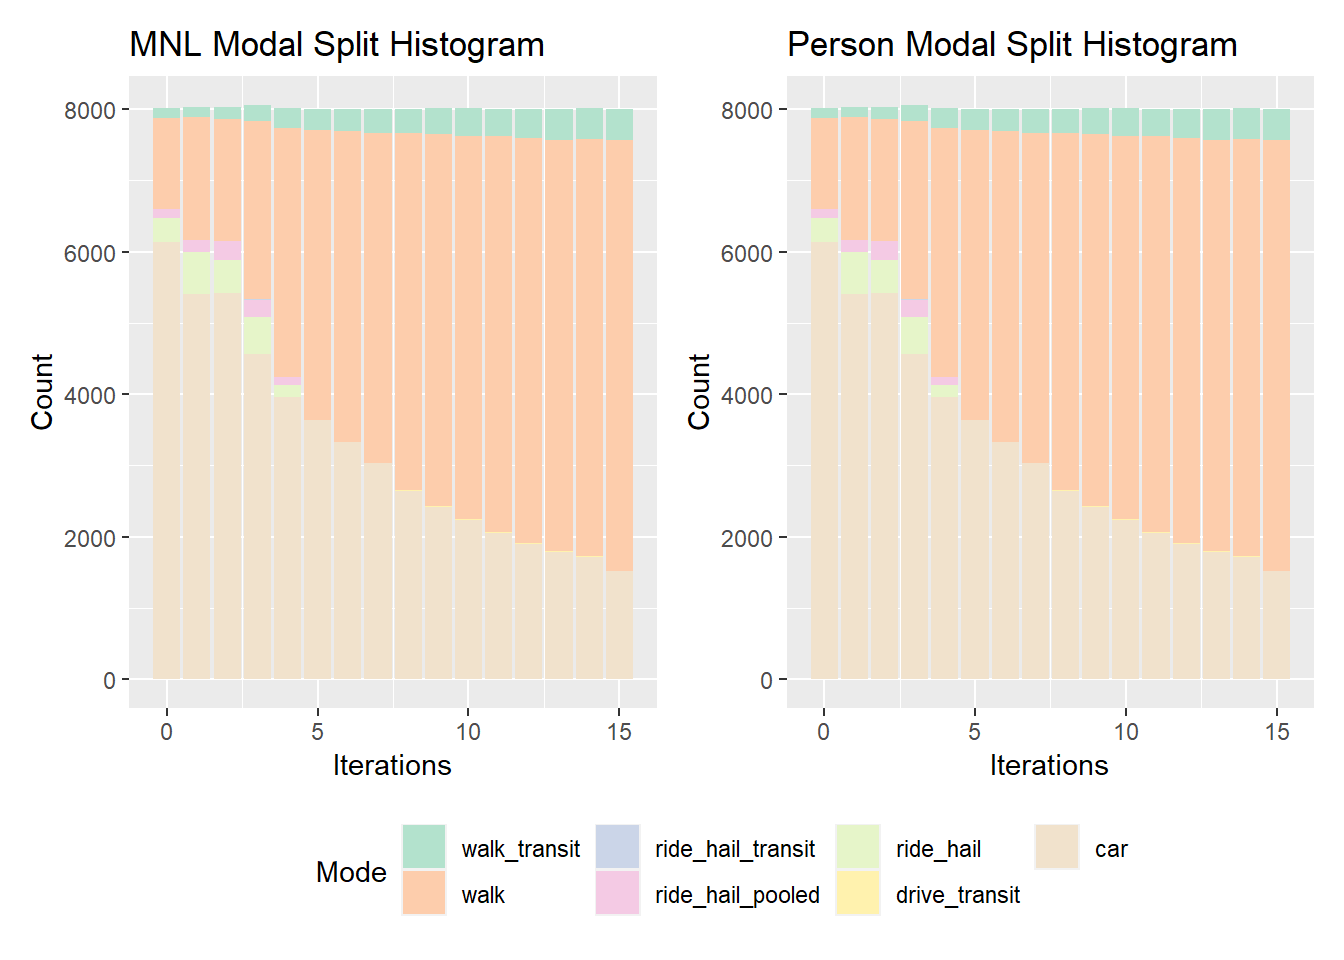
\includegraphics{mode_choice_calibration_files/figure-latex/unnamed-chunk-2-1.pdf}

By examining the graph above, the MNL model seems to be much less accurate than the other models for agents that are auto deficient and auto sufficient. The Path model as well as the All model seem to be closest to the WFRC results in these vehicle ownership categories. As a result, the Path variable has the largest affect on the vehicle ownership modal estimation.

For the no auto category though, the MNL and Path models seem to predict relatively well.The All model however, does not seem to be a very good predictor of modal shares for this category.

\hypertarget{modal-share-by-tour-purpose}{%
\subsection{Modal Share by Tour Purpose}\label{modal-share-by-tour-purpose}}

The modal share by tour purpose provides a more detailed view of how the modes are distributed across the population based on the tour purpose of the agent's trip. The following figure shows the modal share by tour purpose.

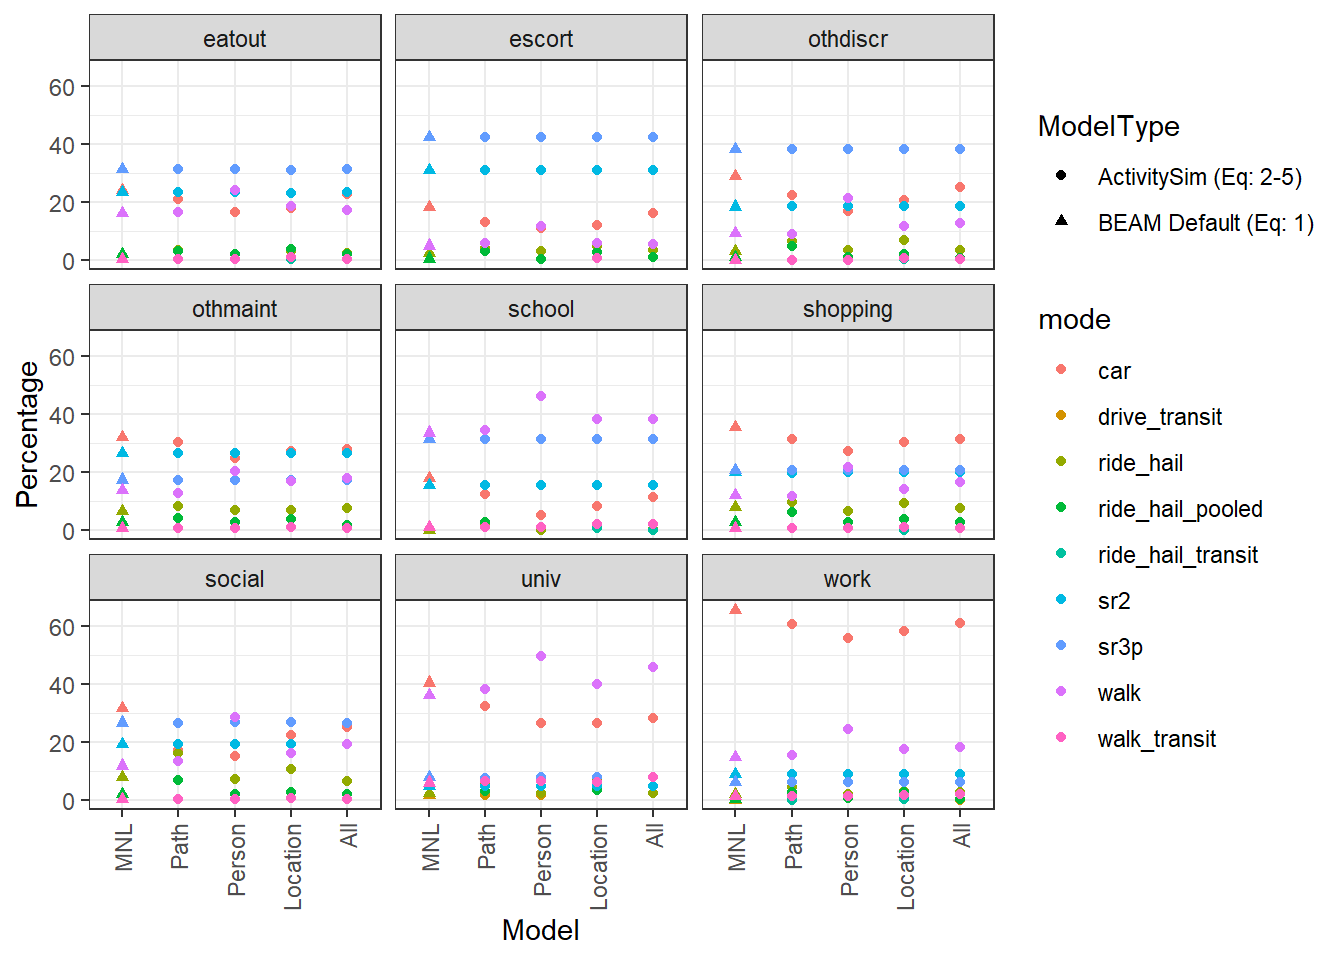
\includegraphics{mode_choice_calibration_files/figure-latex/unnamed-chunk-3-1.pdf}

Unfortunately, the figure above does not include real world data from WFRC. By examing the figure though, it is clear to see that there is a difference in mode choice depending on the tour purpose chosen by the agent. For example, in all the models, car is the highest chosen mode for work trips, whereas for school trips, walking is slightly higher than carpooling and car trips.

\hypertarget{additional-analysis}{%
\subsection{Additional Analysis}\label{additional-analysis}}

Overall, it can be seen that a microsimulation tool with a mode choice structure that mimics that of its parenting activity-based model does not seem to more accurately simulate the distribution of mode choice across a population. This can be verified by examining the comparison modal share graphs; the All model does not seem to most accurately predict actual modal shares.

Although this is true, we see that the variables relating to Person types have the most significant effect in estimating realistic results. The Location and Path variable tyes seemed to predict relatively little in comparison to the Person types. This can be verified by examining the comparison modal share graphs; the Person variable seemed to be the most different when compared to the other factors.

In conclusion, we suggest that future analyzts attempt to rerun a similar scenario that has been presented. Unfortunately, sufficient model calibration was not able to be completed. With a more accurately calibrated scenario, we hypothesize that a microsimulation tool with a mimiced mode choice structure will more accurately simulate the mode choice of a population. We also advise analyzts to pay special attention to Person varaible types, as they have a greater affect in modal decisions than other variable types.

\bibliography{book.bib}


\end{document}

